% Options for packages loaded elsewhere
\PassOptionsToPackage{unicode}{hyperref}
\PassOptionsToPackage{hyphens}{url}
\PassOptionsToPackage{dvipsnames,svgnames*,x11names*}{xcolor}
%
\documentclass[
  11pt,
  a4paper,
]{article}
\usepackage{lmodern}
\usepackage{setspace}
\usepackage{amsmath}
\usepackage{ifxetex,ifluatex}
\ifnum 0\ifxetex 1\fi\ifluatex 1\fi=0 % if pdftex
  \usepackage[T1]{fontenc}
  \usepackage[utf8]{inputenc}
  \usepackage{textcomp} % provide euro and other symbols
  \usepackage{amssymb}
\else % if luatex or xetex
  \usepackage{unicode-math}
  \defaultfontfeatures{Scale=MatchLowercase}
  \defaultfontfeatures[\rmfamily]{Ligatures=TeX,Scale=1}
  \setmainfont[]{Arial}
\fi
% Use upquote if available, for straight quotes in verbatim environments
\IfFileExists{upquote.sty}{\usepackage{upquote}}{}
\IfFileExists{microtype.sty}{% use microtype if available
  \usepackage[]{microtype}
  \UseMicrotypeSet[protrusion]{basicmath} % disable protrusion for tt fonts
}{}
\makeatletter
\@ifundefined{KOMAClassName}{% if non-KOMA class
  \IfFileExists{parskip.sty}{%
    \usepackage{parskip}
  }{% else
    \setlength{\parindent}{0pt}
    \setlength{\parskip}{6pt plus 2pt minus 1pt}}
}{% if KOMA class
  \KOMAoptions{parskip=half}}
\makeatother
\usepackage{xcolor}
\IfFileExists{xurl.sty}{\usepackage{xurl}}{} % add URL line breaks if available
\IfFileExists{bookmark.sty}{\usepackage{bookmark}}{\usepackage{hyperref}}
\hypersetup{
  pdftitle={Livro `Econometria Básica de Gujarati'},
  pdfauthor={Francisco Piccolo},
  colorlinks=true,
  linkcolor=RoyalBlue,
  filecolor=Maroon,
  citecolor=Blue,
  urlcolor=RoyalBlue,
  pdfcreator={LaTeX via pandoc}}
\urlstyle{same} % disable monospaced font for URLs
\usepackage[margin=.5in]{geometry}
\usepackage{longtable,booktabs}
\usepackage{calc} % for calculating minipage widths
% Correct order of tables after \paragraph or \subparagraph
\usepackage{etoolbox}
\makeatletter
\patchcmd\longtable{\par}{\if@noskipsec\mbox{}\fi\par}{}{}
\makeatother
% Allow footnotes in longtable head/foot
\IfFileExists{footnotehyper.sty}{\usepackage{footnotehyper}}{\usepackage{footnote}}
\makesavenoteenv{longtable}
\usepackage{graphicx}
\makeatletter
\def\maxwidth{\ifdim\Gin@nat@width>\linewidth\linewidth\else\Gin@nat@width\fi}
\def\maxheight{\ifdim\Gin@nat@height>\textheight\textheight\else\Gin@nat@height\fi}
\makeatother
% Scale images if necessary, so that they will not overflow the page
% margins by default, and it is still possible to overwrite the defaults
% using explicit options in \includegraphics[width, height, ...]{}
\setkeys{Gin}{width=\maxwidth,height=\maxheight,keepaspectratio}
% Set default figure placement to htbp
\makeatletter
\def\fps@figure{htbp}
\makeatother
\setlength{\emergencystretch}{3em} % prevent overfull lines
\providecommand{\tightlist}{%
  \setlength{\itemsep}{0pt}\setlength{\parskip}{0pt}}
\setcounter{secnumdepth}{-\maxdimen} % remove section numbering
\pagestyle{plain}
\usepackage{lineno,sectsty,color,colortbl,titling} % add

% Left justification of the text: see https://www.sharelatex.com/learn/Text_alignment
% \usepackage[document]{ragged2e} % already in the latex template
\newcommand{\bleft}{\begin{flushleft}}
\newcommand{\eleft}{\end{flushleft}}
\allsectionsfont{\mdseries\bfseries\color{RoyalBlue}}
\pretitle{\begin{center}\LARGE\color{RoyalBlue}}
\usepackage{booktabs}
\usepackage{longtable}
\usepackage{array}
\usepackage{multirow}
\usepackage{wrapfig}
\usepackage{float}
\usepackage{colortbl}
\usepackage{pdflscape}
\usepackage{tabu}
\usepackage{threeparttable}
\usepackage{threeparttablex}
\usepackage[normalem]{ulem}
\usepackage{makecell}
\usepackage{xcolor}
\ifluatex
  \usepackage{selnolig}  % disable illegal ligatures
\fi

\title{Livro `Econometria Básica de Gujarati'}
\usepackage{etoolbox}
\makeatletter
\providecommand{\subtitle}[1]{% add subtitle to \maketitle
  \apptocmd{\@title}{\par {\large #1 \par}}{}{}
}
\makeatother
\subtitle{Resolvendo Exercícios Propostos}
\author{Francisco Piccolo}
\date{2020-03-10}

\begin{document}
\maketitle

\setstretch{1.2}
Neste post vou resolver alguns exercícios de um livro de econometria bastante usado nos cursos de economia, que se chama \href{https://www.amazon.com.br/Econometria-B\%C3\%A1sica-Damodar-N-Gujarati/dp/8563308327/ref=sr_1_1?__mk_pt_BR=\%C3\%85M\%C3\%85\%C5\%BD\%C3\%95\%C3\%91\&dchild=1\&keywords=econometria+b\%C3\%A1sica+gujarati\&qid=1624149011\&sr=8-1}{Econometria Básica} de Gujarati. Os códigos usados nos exercícios podem ser encontrados no arquivo .Rmd que gera este PDF neste \href{https://github.com/FranciscoPiccolo/franciscopiccolo.github.io/blob/master/02.solving_exercises_from_gujarati's_book_basic_econometrics_20200301/article.Rmd}{link}. Os datasets dos exercícios também estarão no meu repositório do Github neste \href{https://github.com/FranciscoPiccolo/franciscopiccolo.github.io/tree/master/02.solving_exercises_from_gujarati's_book_basic_econometrics_20200301/datasets}{link}.

O foco será na resolução dos exercícios que permitem aplicações com o R, que serão na maior parte os que pedem para plotar um gráfico ou fazer uma regressão e interpretar os resultados.

\hypertarget{capuxedtulo-1---a-natureza-da-anuxe1lise-de-regressuxe3o}{%
\section{Capítulo 1 - A Natureza da Análise de Regressão}\label{capuxedtulo-1---a-natureza-da-anuxe1lise-de-regressuxe3o}}

\hypertarget{a-tabela-1.3-apresenta-dados-relativos-ao-uxedndice-de-preuxe7os-ao-consumidor-cpi-de-sete-pauxedses-industrializados.-a-base-do-uxedndice-uxe9-19821984-100.}{%
\subsubsection{1.1. A Tabela 1.3 apresenta dados relativos ao Índice de Preços ao Consumidor (CPI) de sete países industrializados. A base do índice é 1982--1984 = 100.}\label{a-tabela-1.3-apresenta-dados-relativos-ao-uxedndice-de-preuxe7os-ao-consumidor-cpi-de-sete-pauxedses-industrializados.-a-base-do-uxedndice-uxe9-19821984-100.}}

\begin{table}[H]

\caption{\label{tab:unnamed-chunk-3}Amostra do Dataset}
\centering
\fontsize{10}{12}\selectfont
\begin{tabular}[t]{lrrrrrrr}
\toprule
\cellcolor{RoyalBlue}{\textcolor{white}{\textbf{year}}} & \cellcolor{RoyalBlue}{\textcolor{white}{\textbf{usa}}} & \cellcolor{RoyalBlue}{\textcolor{white}{\textbf{canada}}} & \cellcolor{RoyalBlue}{\textcolor{white}{\textbf{japan}}} & \cellcolor{RoyalBlue}{\textcolor{white}{\textbf{france}}} & \cellcolor{RoyalBlue}{\textcolor{white}{\textbf{germany}}} & \cellcolor{RoyalBlue}{\textcolor{white}{\textbf{italy}}} & \cellcolor{RoyalBlue}{\textcolor{white}{\textbf{uk}}}\\
\midrule
1980 & 824 & 761 & 910 & 722 & 867 & 639 & 785\\
\addlinespace
1981 & 909 & 856 & 953 & 818 & 922 & 755 & 879\\
\addlinespace
1982 & 965 & 949 & 981 & 917 & 970 & 878 & 954\\
\addlinespace
1983 & 996 & 1.004 & 998 & 1.003 & 1.003 & 1.008 & 998\\
\addlinespace
1984 & 1.039 & 1.047 & 1.021 & 1.080 & 1.027 & 1.114 & 1.048\\
\bottomrule
\end{tabular}
\end{table}

\textbf{b. Represente graficamente a taxa de inflação de cada país em relação ao tempo (isto é, use o eixo horizontal para o tempo e o eixo vertical para a taxa de inflação).}

\begin{center}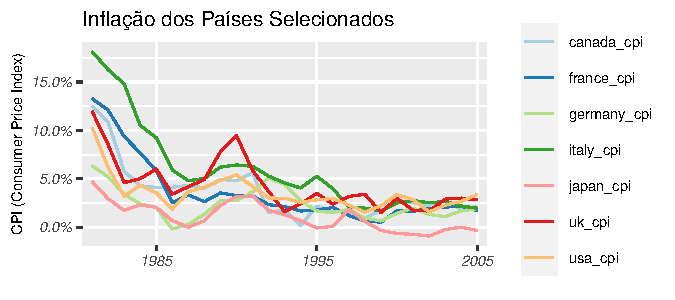
\includegraphics{article_files/figure-latex/unnamed-chunk-5-1} \end{center}

\hypertarget{section}{%
\subsubsection{1.2}\label{section}}

\textbf{a. Usando a Tabela 1.3, represente as taxas de inflação do Canadá, França, Alemanha, Itália, Japão e Reino Unido em relação à taxa de inflação dos Estados Unidos.}

Com o pacote \textbf{GGally} é possível criar estes comparativos mais facilmente.

\begin{center}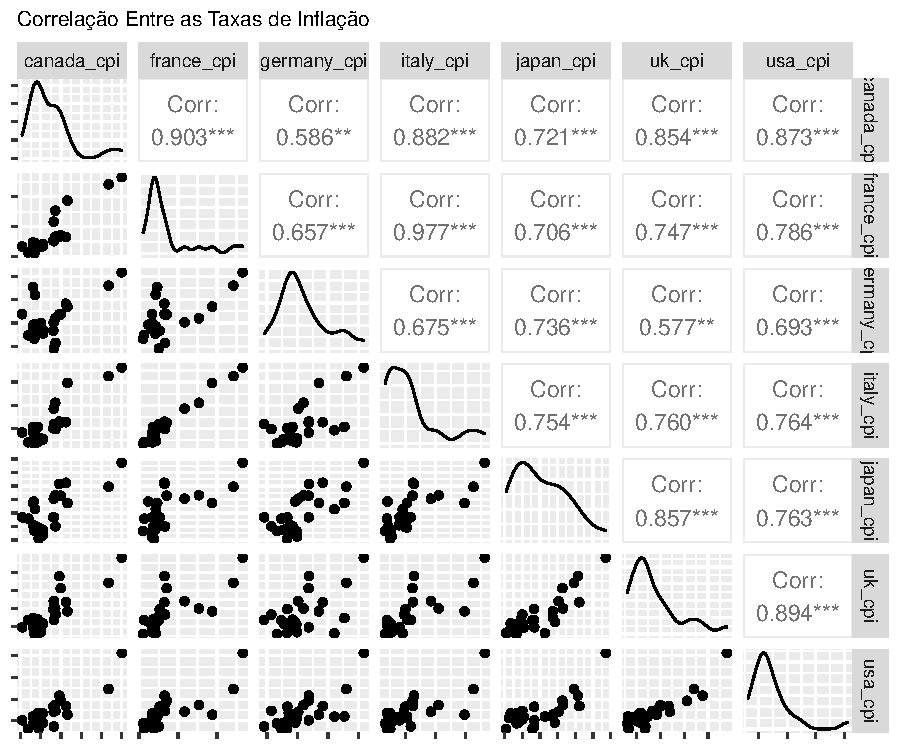
\includegraphics{article_files/figure-latex/unnamed-chunk-6-1} \end{center}

Apenas a linha e coluna `usa\_cpi' precisa ser usada, mostrando o gráficos de dispersão entre as variáveis e seu coeficiente de correlação. A menor correlação é a da Alemanha, que ficou em 69,3\%.

\hypertarget{a-tabela-1.4-apresenta-as-taxas-de-cuxe2mbio-em-sete-pauxedses-industrializados-no-peruxedodo-1985---2006.-exceto-no-caso-do-reino-unido-as-taxas-de-cuxe2mbio-estuxe3o-definidas-como-unidades-de-moeda-estrangeira-por-um-duxf3lar-no-caso-do-reino-unido-a-taxa-de-cuxe2mbio-uxe9-dada-como-o-nuxfamero-de-duxf3lares-por-uma-libra-esterlina.}{%
\subsubsection{1.3 A Tabela 1.4 apresenta as taxas de câmbio em sete países industrializados, no período 1985 - 2006. Exceto no caso do Reino Unido, as taxas de câmbio estão definidas como unidades de moeda estrangeira por um dólar; no caso do Reino Unido, a taxa de câmbio é dada como o número de dólares por uma libra esterlina.}\label{a-tabela-1.4-apresenta-as-taxas-de-cuxe2mbio-em-sete-pauxedses-industrializados-no-peruxedodo-1985---2006.-exceto-no-caso-do-reino-unido-as-taxas-de-cuxe2mbio-estuxe3o-definidas-como-unidades-de-moeda-estrangeira-por-um-duxf3lar-no-caso-do-reino-unido-a-taxa-de-cuxe2mbio-uxe9-dada-como-o-nuxfamero-de-duxf3lares-por-uma-libra-esterlina.}}

\begin{table}[H]

\caption{\label{tab:unnamed-chunk-7}Amostra do Dataset}
\centering
\fontsize{10}{12}\selectfont
\begin{tabular}[t]{lrrrlrrrrr}
\toprule
\cellcolor{RoyalBlue}{\textcolor{white}{\textbf{Ano}}} & \cellcolor{RoyalBlue}{\textcolor{white}{\textbf{Australia}}} & \cellcolor{RoyalBlue}{\textcolor{white}{\textbf{Canada}}} & \cellcolor{RoyalBlue}{\textcolor{white}{\textbf{China}}} & \cellcolor{RoyalBlue}{\textcolor{white}{\textbf{Japao}}} & \cellcolor{RoyalBlue}{\textcolor{white}{\textbf{Mexico}}} & \cellcolor{RoyalBlue}{\textcolor{white}{\textbf{Coreia.sul}}} & \cellcolor{RoyalBlue}{\textcolor{white}{\textbf{Suecia}}} & \cellcolor{RoyalBlue}{\textcolor{white}{\textbf{Suica}}} & \cellcolor{RoyalBlue}{\textcolor{white}{\textbf{Reino.unido}}}\\
\midrule
1985 & 0,7003 & 1,3659 & 2,9434 & 238.4700 & 0,257 & 872,45 & 8,6032 & 2,4552 & 1,2974\\
\addlinespace
1986 & 0,6709 & 1,3896 & 3,4616 & 168.3500 & 0,612 & 884,60 & 7,1273 & 1,7979 & 1,4677\\
\addlinespace
1987 & 0,7014 & 1,3259 & 3,7314 & 144.6000 & 1,378 & 826,16 & 6,3469 & 1,4918 & 1,6398\\
\addlinespace
1988 & 0,7841 & 1,2306 & 3,7314 & 128.1700 & 2,273 & 734,52 & 6,1370 & 1,4643 & 1,7813\\
\addlinespace
1989 & 0,7919 & 1,1842 & 3,7673 & 138.0700 & 2,461 & 674,13 & 6,4559 & 1,6369 & 1,6382\\
\bottomrule
\end{tabular}
\end{table}

\textbf{a. Represente graficamente a evolução das taxas de câmbio ao longo do tempo e comente sobre o comportamento geral dessa evolução.}

\begin{center}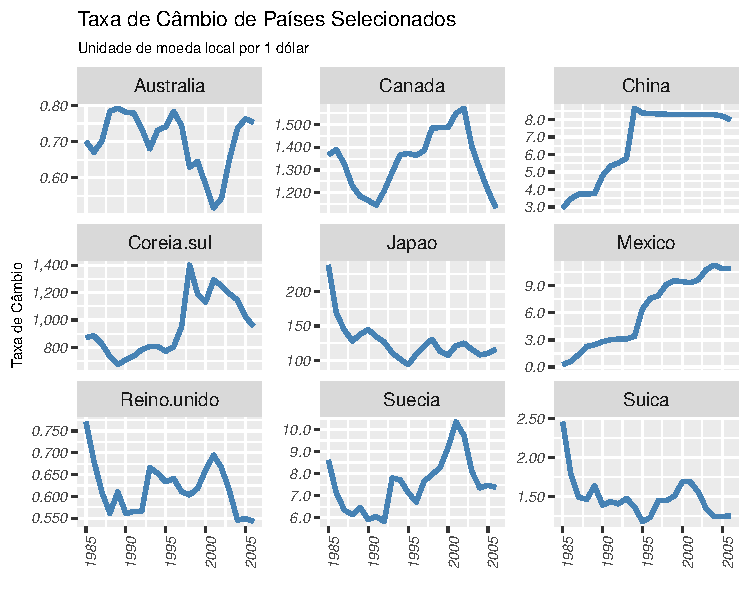
\includegraphics{article_files/figure-latex/unnamed-chunk-8-1} \end{center}

\hypertarget{os-dados-apresentados-na-tabela-1.6-foram-divulgados-na-ediuxe7uxe3o-do-the-wall-street-journal-de-1uxba-de-maruxe7o-de-1984.-os-dados-relacionam-o-oruxe7amento-de-publicidade-em-milhuxf5es-de-duxf3lares-de-21-empresas-em-1983-com-as-impressuxf5es-retidas-semanalmente-pelos-que-viram-os-produtos-anunciados-por-essas-empresas.-os-dados-foram-obtidos-em-uma-pesquisa-realizada-com-4-mil-adultos-em-que-foi-pedido-aos-usuuxe1rios-dos-produtos-que-citassem-um-comercial-da-categoria-do-produto-que-tivessem-assistido-na-semana-anterior.}{%
\subsubsection{1.7 Os dados apresentados na Tabela 1.6 foram divulgados na edição do The Wall Street Journal de 1º de março de 1984. Os dados relacionam o orçamento de publicidade (em milhões de dólares) de 21 empresas em 1983 com as impressões retidas, semanalmente, pelos que viram os produtos anunciados por essas empresas. Os dados foram obtidos em uma pesquisa realizada com 4 mil adultos, em que foi pedido aos usuários dos produtos que citassem um comercial da categoria do produto que tivessem assistido na semana anterior.}\label{os-dados-apresentados-na-tabela-1.6-foram-divulgados-na-ediuxe7uxe3o-do-the-wall-street-journal-de-1uxba-de-maruxe7o-de-1984.-os-dados-relacionam-o-oruxe7amento-de-publicidade-em-milhuxf5es-de-duxf3lares-de-21-empresas-em-1983-com-as-impressuxf5es-retidas-semanalmente-pelos-que-viram-os-produtos-anunciados-por-essas-empresas.-os-dados-foram-obtidos-em-uma-pesquisa-realizada-com-4-mil-adultos-em-que-foi-pedido-aos-usuuxe1rios-dos-produtos-que-citassem-um-comercial-da-categoria-do-produto-que-tivessem-assistido-na-semana-anterior.}}

\begin{table}[H]

\caption{\label{tab:unnamed-chunk-9}Amostra do Dataset}
\centering
\fontsize{10}{12}\selectfont
\begin{tabular}[t]{rrl}
\toprule
\cellcolor{RoyalBlue}{\textcolor{white}{\textbf{impressions}}} & \cellcolor{RoyalBlue}{\textcolor{white}{\textbf{investment}}} & \cellcolor{RoyalBlue}{\textcolor{white}{\textbf{company}}}\\
\midrule
32,1 & 50,1 & Miller\_Lite\\
\addlinespace
99,6 & 74,1 & Pepsi\\
\addlinespace
11,7 & 19,3 & Stroh\\
\addlinespace
21,9 & 22,9 & Fed\_Express\\
\addlinespace
60,8 & 82,4 & Burger\_King\\
\bottomrule
\end{tabular}
\end{table}

\newpage

\textbf{a. Trace um gráfico com as impressões no eixo vertical e os gastos com publicidade no eixo horizontal.}

\begin{center}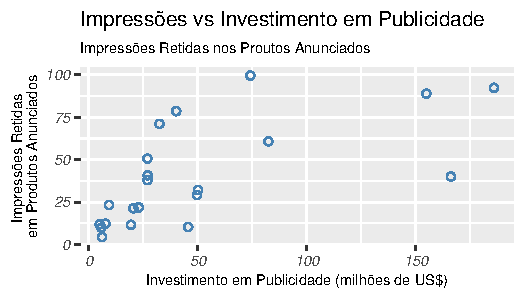
\includegraphics{article_files/figure-latex/unnamed-chunk-10-1} \end{center}

\newpage

\hypertarget{capuxedtulo-2---anuxe1lise-de-regressuxe3o-com-duas-variuxe1veis-algumas-ideias-buxe1sicas}{%
\section{Capítulo 2 - Análise de Regressão com Duas Variáveis: Algumas Ideias Básicas}\label{capuxedtulo-2---anuxe1lise-de-regressuxe3o-com-duas-variuxe1veis-algumas-ideias-buxe1sicas}}

\hypertarget{com-os-dados-da-tabela-2.7-relativos-aos-estados-unidos-nos-peruxedodo-1980-2006}{%
\subsubsection{2.14. Com os dados da Tabela 2.7 relativos aos Estados Unidos nos período 1980-2006:}\label{com-os-dados-da-tabela-2.7-relativos-aos-estados-unidos-nos-peruxedodo-1980-2006}}

\begin{table}[H]

\caption{\label{tab:unnamed-chunk-11}Amostra do Dataset}
\centering
\fontsize{10}{12}\selectfont
\resizebox{\linewidth}{!}{
\begin{tabular}[t]{rrrrrrr}
\toprule
\cellcolor{RoyalBlue}{\textcolor{white}{\textbf{year}}} & \cellcolor{RoyalBlue}{\textcolor{white}{\textbf{share\_men\_work\_force}}} & \cellcolor{RoyalBlue}{\textcolor{white}{\textbf{share\_women\_work\_force}}} & \cellcolor{RoyalBlue}{\textcolor{white}{\textbf{unemployment\_men}}} & \cellcolor{RoyalBlue}{\textcolor{white}{\textbf{unemployment\_women}}} & \cellcolor{RoyalBlue}{\textcolor{white}{\textbf{avg\_hourly\_earning\_men}}} & \cellcolor{RoyalBlue}{\textcolor{white}{\textbf{avg\_hourly\_earning\_women}}}\\
\midrule
1.980 & 77,4 & 51,5 & 6,9 & 7,4 & 7,99 & 6,84\\
\addlinespace
1.981 & 77,0 & 52,1 & 7,4 & 7,9 & 7,88 & 7,43\\
\addlinespace
1.982 & 76,6 & 52,6 & 9,9 & 9,4 & 7,86 & 7,86\\
\addlinespace
1.983 & 76,4 & 52,9 & 9,9 & 9,2 & 7,95 & 8,19\\
\addlinespace
1.984 & 76,4 & 53,6 & 7,4 & 7,6 & 7,95 & 8,48\\
\bottomrule
\end{tabular}}
\end{table}

\textbf{a. Represente graficamente a relação entre a taxa de participação dos homens na força de trabalho civil e a taxa de desemprego civil dos homens. Trace, a olho, uma linha de regressão que passe pelos pontos. A priori, qual a relação esperada entre as duas variáveis e em que teoria econômica está embasada? O diagrama de dispersão respalda essa teoria?}

\begin{center}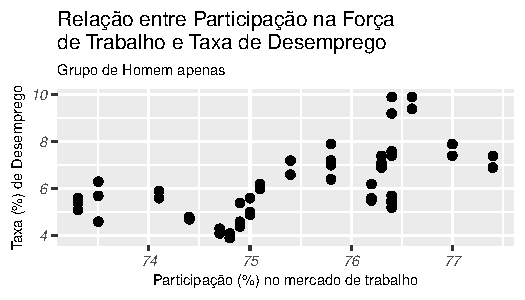
\includegraphics{article_files/figure-latex/unnamed-chunk-13-1} \end{center}

\textbf{b. Faça o mesmo para as mulheres}

\begin{center}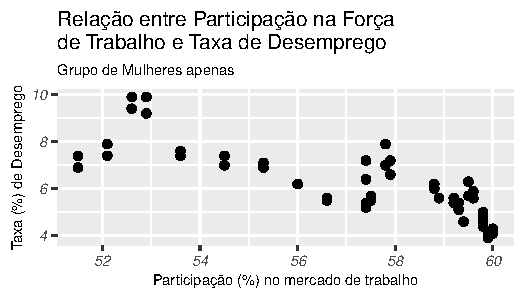
\includegraphics{article_files/figure-latex/unnamed-chunk-14-1} \end{center}

\textbf{c.~Agora, represente graficamente a taxa de participação de homens e mulheres em relação aos ganhos médios por hora (em dólares de 1982). (Você pode usar gráficos separados.) O que constatou? Como você justificaria isso?}

\begin{center}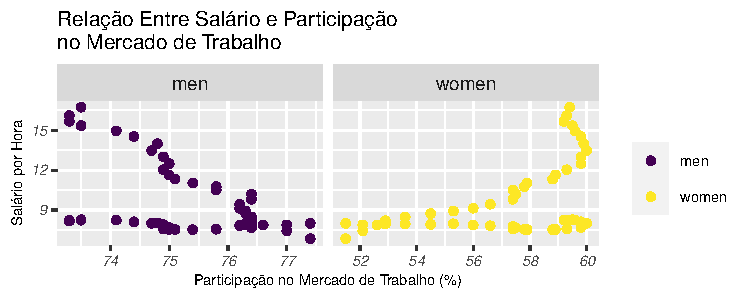
\includegraphics{article_files/figure-latex/unnamed-chunk-15-1} \end{center}

\hypertarget{a-tabela-2.8-apresenta-dados-sobre-despesas-com-alimentauxe7uxe3o-e-gastos-totais-em-rupias-para-uma-amostra-de-55-domicuxedlios-rurais-da-uxedndia.-no-inuxedcio-de-2000-um-duxf3lar-americano-era-equivalente-a-cerca-de-40-rupias-indianas.}{%
\subsubsection{2.15. A Tabela 2.8 apresenta dados sobre despesas com alimentação e gastos totais, em rupias, para uma amostra de 55 domicílios rurais da Índia. (No início de 2000, um dólar americano era equivalente a cerca de 40 rupias indianas.)}\label{a-tabela-2.8-apresenta-dados-sobre-despesas-com-alimentauxe7uxe3o-e-gastos-totais-em-rupias-para-uma-amostra-de-55-domicuxedlios-rurais-da-uxedndia.-no-inuxedcio-de-2000-um-duxf3lar-americano-era-equivalente-a-cerca-de-40-rupias-indianas.}}

\begin{table}[H]

\caption{\label{tab:unnamed-chunk-16}Amostra do Dataset}
\centering
\fontsize{10}{12}\selectfont
\begin{tabular}[t]{rr}
\toprule
\cellcolor{RoyalBlue}{\textcolor{white}{\textbf{food}}} & \cellcolor{RoyalBlue}{\textcolor{white}{\textbf{total}}}\\
\midrule
217 & 382\\
\addlinespace
196 & 388\\
\addlinespace
303 & 391\\
\addlinespace
270 & 415\\
\addlinespace
325 & 456\\
\bottomrule
\end{tabular}
\end{table}

\textbf{a. Represente graficamente os dados colocando no eixo vertical as despesas com alimentação e no eixo horizontal os gastos totais. Trace uma linha de regressão.}

\begin{center}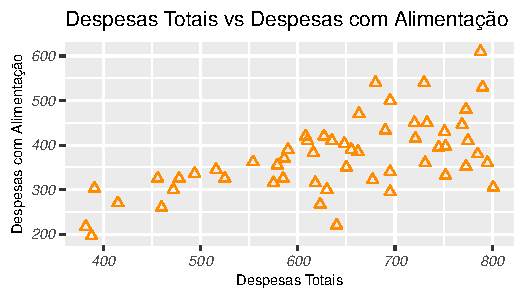
\includegraphics{article_files/figure-latex/unnamed-chunk-17-1} \end{center}

\hypertarget{a-tabela-2.9-apresenta-dados-sobre-a-pontuauxe7uxe3o-muxe9dia-do-teste-de-aptiduxe3o-escolar-sat-para-os-estudantes-que-se-preparavam-para-ingressar-no-ensino-superior-no-peruxedodo-1967-1990.}{%
\subsubsection{2.16. A Tabela 2.9 apresenta dados sobre a pontuação média do Teste de Aptidão Escolar (SAT) para os estudantes que se preparavam para ingressar no ensino superior no período 1967-1990.}\label{a-tabela-2.9-apresenta-dados-sobre-a-pontuauxe7uxe3o-muxe9dia-do-teste-de-aptiduxe3o-escolar-sat-para-os-estudantes-que-se-preparavam-para-ingressar-no-ensino-superior-no-peruxedodo-1967-1990.}}

\begin{table}[H]

\caption{\label{tab:unnamed-chunk-18}Amostra do Dataset}
\centering
\fontsize{10}{12}\selectfont
\resizebox{\linewidth}{!}{
\begin{tabular}[t]{rrrrrrr}
\toprule
\cellcolor{RoyalBlue}{\textcolor{white}{\textbf{year}}} & \cellcolor{RoyalBlue}{\textcolor{white}{\textbf{men\_verbal\_score}}} & \cellcolor{RoyalBlue}{\textcolor{white}{\textbf{wonem\_verbal\_score}}} & \cellcolor{RoyalBlue}{\textcolor{white}{\textbf{verbal\_score\_total}}} & \cellcolor{RoyalBlue}{\textcolor{white}{\textbf{men\_math\_score}}} & \cellcolor{RoyalBlue}{\textcolor{white}{\textbf{women\_math\_score}}} & \cellcolor{RoyalBlue}{\textcolor{white}{\textbf{math\_score\_total}}}\\
\midrule
1.972 & 531 & 529 & 530 & 527 & 489 & 509\\
\addlinespace
1.973 & 523 & 521 & 523 & 525 & 489 & 506\\
\addlinespace
1.974 & 524 & 520 & 521 & 524 & 488 & 505\\
\addlinespace
1.975 & 515 & 509 & 512 & 518 & 479 & 498\\
\addlinespace
1.976 & 511 & 508 & 509 & 520 & 475 & 497\\
\bottomrule
\end{tabular}}
\end{table}

\textbf{a. Use o eixo horizontal para os anos e o eixo vertical para a pontuação obtida para traçar as notas nas provas de aptidão verbal e matemática obtidas por homens e mulheres, separadamente.}

\begin{center}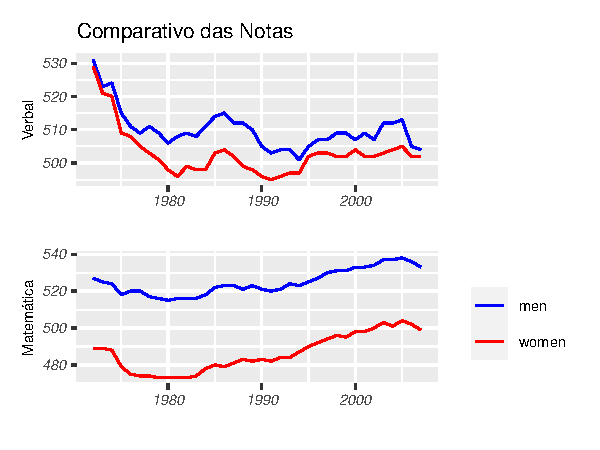
\includegraphics{article_files/figure-latex/unnamed-chunk-19-1} \end{center}

\textbf{d.~Represente graficamente as notas de matemática das mulheres em relação às dos homens. O que você observa?}

\begin{center}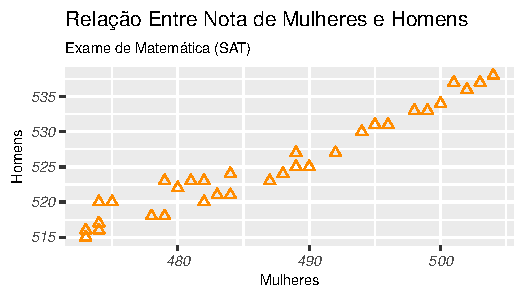
\includegraphics{article_files/figure-latex/unnamed-chunk-20-1} \end{center}

\newpage

\hypertarget{capuxedtulo-3---modelo-de-regressuxe3o-de-duas-variuxe1veis-o-problema-da-estimauxe7uxe3o}{%
\section{Capítulo 3 - Modelo de Regressão de Duas Variáveis: O Problema da Estimação}\label{capuxedtulo-3---modelo-de-regressuxe3o-de-duas-variuxe1veis-o-problema-da-estimauxe7uxe3o}}

\hypertarget{na-tabela-3.5-estuxe1-a-classificauxe7uxe3o-de-dez-estudantes-nas-provas-parcial-e-final-de-estatuxedstica.-calcule-o-coeficiente-de-correlauxe7uxe3o-de-rankings-de-spearman-e-interprete-os-resultados.}{%
\subsubsection{3.18. Na Tabela 3.5 está a classificação de dez estudantes nas provas parcial e final de estatística. Calcule o coeficiente de correlação de rankings de Spearman e interprete os resultados.**}\label{na-tabela-3.5-estuxe1-a-classificauxe7uxe3o-de-dez-estudantes-nas-provas-parcial-e-final-de-estatuxedstica.-calcule-o-coeficiente-de-correlauxe7uxe3o-de-rankings-de-spearman-e-interprete-os-resultados.}}

\begin{table}[H]

\caption{\label{tab:unnamed-chunk-21}Amostra do Dataset}
\centering
\fontsize{10}{12}\selectfont
\begin{tabular}[t]{rrl}
\toprule
\cellcolor{RoyalBlue}{\textcolor{white}{\textbf{parcial\_test}}} & \cellcolor{RoyalBlue}{\textcolor{white}{\textbf{final\_test}}} & \cellcolor{RoyalBlue}{\textcolor{white}{\textbf{student}}}\\
\midrule
1 & 3 & a\\
\addlinespace
3 & 2 & b\\
\addlinespace
7 & 8 & c\\
\addlinespace
10 & 7 & d\\
\addlinespace
9 & 9 & e\\
\addlinespace
5 & 6 & f\\
\addlinespace
4 & 5 & g\\
\addlinespace
8 & 10 & h\\
\addlinespace
2 & 1 & i\\
\addlinespace
6 & 4 & j\\
\bottomrule
\end{tabular}
\end{table}

\begin{longtable}[]{@{}cccc@{}}
\caption{Spearman's rank correlation rho: \texttt{table\_3.5\$parcial\_test} and \texttt{table\_3.5\$final\_test}}\tabularnewline
\toprule
\begin{minipage}[b]{(\columnwidth - 3\tabcolsep) * \real{0.24}}\centering
Test statistic\strut
\end{minipage} & \begin{minipage}[b]{(\columnwidth - 3\tabcolsep) * \real{0.21}}\centering
P value\strut
\end{minipage} & \begin{minipage}[b]{(\columnwidth - 3\tabcolsep) * \real{0.35}}\centering
Alternative hypothesis\strut
\end{minipage} & \begin{minipage}[b]{(\columnwidth - 3\tabcolsep) * \real{0.12}}\centering
rho\strut
\end{minipage}\tabularnewline
\midrule
\endfirsthead
\toprule
\begin{minipage}[b]{(\columnwidth - 3\tabcolsep) * \real{0.24}}\centering
Test statistic\strut
\end{minipage} & \begin{minipage}[b]{(\columnwidth - 3\tabcolsep) * \real{0.21}}\centering
P value\strut
\end{minipage} & \begin{minipage}[b]{(\columnwidth - 3\tabcolsep) * \real{0.35}}\centering
Alternative hypothesis\strut
\end{minipage} & \begin{minipage}[b]{(\columnwidth - 3\tabcolsep) * \real{0.12}}\centering
rho\strut
\end{minipage}\tabularnewline
\midrule
\endhead
\begin{minipage}[t]{(\columnwidth - 3\tabcolsep) * \real{0.24}}\centering
26\strut
\end{minipage} & \begin{minipage}[t]{(\columnwidth - 3\tabcolsep) * \real{0.21}}\centering
0.004459 * *\strut
\end{minipage} & \begin{minipage}[t]{(\columnwidth - 3\tabcolsep) * \real{0.35}}\centering
two.sided\strut
\end{minipage} & \begin{minipage}[t]{(\columnwidth - 3\tabcolsep) * \real{0.12}}\centering
0.8424\strut
\end{minipage}\tabularnewline
\bottomrule
\end{longtable}

\hypertarget{a-tabela-3.6-apresenta-dados-relativos-a-uxedndices-de-produuxe7uxe3o-por-hora-x-e-remunerauxe7uxe3o-real-por-hora-y-para-os-setores-empresarial-e-empresarial-nuxe3o-agruxedcola-da-economia-dos-estados-unidos-no-peruxedodo-1960-2005.-o-ano-base-dos-uxedndices-uxe9-1992-d-100-e-os-uxedndices-foram-ajustados-sazonalmente}{%
\subsubsection{3.20. A Tabela 3.6 apresenta dados relativos a índices de produção por hora (X) e remuneração real por hora (Y) para os setores empresarial e empresarial não agrícola da economia dos Estados Unidos no período 1960-2005. O ano-base dos índices é 1992 D 100 e os índices foram ajustados sazonalmente**}\label{a-tabela-3.6-apresenta-dados-relativos-a-uxedndices-de-produuxe7uxe3o-por-hora-x-e-remunerauxe7uxe3o-real-por-hora-y-para-os-setores-empresarial-e-empresarial-nuxe3o-agruxedcola-da-economia-dos-estados-unidos-no-peruxedodo-1960-2005.-o-ano-base-dos-uxedndices-uxe9-1992-d-100-e-os-uxedndices-foram-ajustados-sazonalmente}}

\begin{table}[H]

\caption{\label{tab:unnamed-chunk-23}Amostra do Dataset}
\centering
\fontsize{10}{12}\selectfont
\begin{tabular}[t]{rrrrr}
\toprule
\cellcolor{RoyalBlue}{\textcolor{white}{\textbf{year}}} & \cellcolor{RoyalBlue}{\textcolor{white}{\textbf{corporate}}} & \cellcolor{RoyalBlue}{\textcolor{white}{\textbf{corporate\_wages}}} & \cellcolor{RoyalBlue}{\textcolor{white}{\textbf{non\_agricultural}}} & \cellcolor{RoyalBlue}{\textcolor{white}{\textbf{non\_agricultural\_wages}}}\\
\midrule
1.960 & 48,9 & 60,8 & 51,9 & 63,3\\
\addlinespace
1.961 & 50,6 & 62,5 & 53,5 & 64,8\\
\addlinespace
1.962 & 52,9 & 64,6 & 55,9 & 66,7\\
\addlinespace
1.963 & 55,0 & 66,1 & 57,8 & 68,1\\
\addlinespace
1.964 & 56,8 & 67,7 & 59,6 & 69,3\\
\bottomrule
\end{tabular}
\end{table}

\newpage

\textbf{a. Represente graficamente Y contra X para os dois setores da economia separadamente.}

\begin{center}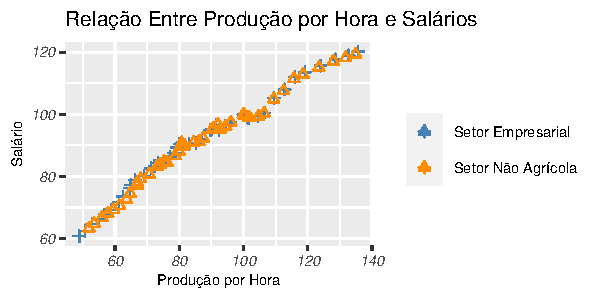
\includegraphics{article_files/figure-latex/unnamed-chunk-24-1} \end{center}

\textbf{c.~Estime uma regressão de MQO de Y contra X. Guarde os resultados para examiná-los novamente depois de estudar o Capítulo 5.}

Cada setor terá uma regressão estimada.

\begin{itemize}
\tightlist
\item
  Setor Empresarial
\end{itemize}

\begin{longtable}[]{@{}ccccc@{}}
\toprule
\begin{minipage}[b]{(\columnwidth - 4\tabcolsep) * \real{0.25}}\centering
~\strut
\end{minipage} & \begin{minipage}[b]{(\columnwidth - 4\tabcolsep) * \real{0.15}}\centering
Estimate\strut
\end{minipage} & \begin{minipage}[b]{(\columnwidth - 4\tabcolsep) * \real{0.18}}\centering
Std. Error\strut
\end{minipage} & \begin{minipage}[b]{(\columnwidth - 4\tabcolsep) * \real{0.14}}\centering
t value\strut
\end{minipage} & \begin{minipage}[b]{(\columnwidth - 4\tabcolsep) * \real{0.17}}\centering
Pr(\textgreater\textbar t\textbar)\strut
\end{minipage}\tabularnewline
\midrule
\endhead
\begin{minipage}[t]{(\columnwidth - 4\tabcolsep) * \real{0.25}}\centering
\textbf{(Intercept)}\strut
\end{minipage} & \begin{minipage}[t]{(\columnwidth - 4\tabcolsep) * \real{0.15}}\centering
32.74\strut
\end{minipage} & \begin{minipage}[t]{(\columnwidth - 4\tabcolsep) * \real{0.18}}\centering
1.394\strut
\end{minipage} & \begin{minipage}[t]{(\columnwidth - 4\tabcolsep) * \real{0.14}}\centering
23.49\strut
\end{minipage} & \begin{minipage}[t]{(\columnwidth - 4\tabcolsep) * \real{0.17}}\centering
1.584e-26\strut
\end{minipage}\tabularnewline
\begin{minipage}[t]{(\columnwidth - 4\tabcolsep) * \real{0.25}}\centering
\textbf{corporate}\strut
\end{minipage} & \begin{minipage}[t]{(\columnwidth - 4\tabcolsep) * \real{0.15}}\centering
0.6704\strut
\end{minipage} & \begin{minipage}[t]{(\columnwidth - 4\tabcolsep) * \real{0.18}}\centering
0.01567\strut
\end{minipage} & \begin{minipage}[t]{(\columnwidth - 4\tabcolsep) * \real{0.14}}\centering
42.78\strut
\end{minipage} & \begin{minipage}[t]{(\columnwidth - 4\tabcolsep) * \real{0.17}}\centering
1.724e-37\strut
\end{minipage}\tabularnewline
\bottomrule
\end{longtable}

\begin{longtable}[]{@{}cccc@{}}
\caption{Fitting linear model: ``corporate\_wages \textasciitilde{} corporate''}\tabularnewline
\toprule
\begin{minipage}[b]{(\columnwidth - 3\tabcolsep) * \real{0.21}}\centering
Observations\strut
\end{minipage} & \begin{minipage}[b]{(\columnwidth - 3\tabcolsep) * \real{0.31}}\centering
Residual Std. Error\strut
\end{minipage} & \begin{minipage}[b]{(\columnwidth - 3\tabcolsep) * \real{0.12}}\centering
\(R^2\)\strut
\end{minipage} & \begin{minipage}[b]{(\columnwidth - 3\tabcolsep) * \real{0.24}}\centering
Adjusted \(R^2\)\strut
\end{minipage}\tabularnewline
\midrule
\endfirsthead
\toprule
\begin{minipage}[b]{(\columnwidth - 3\tabcolsep) * \real{0.21}}\centering
Observations\strut
\end{minipage} & \begin{minipage}[b]{(\columnwidth - 3\tabcolsep) * \real{0.31}}\centering
Residual Std. Error\strut
\end{minipage} & \begin{minipage}[b]{(\columnwidth - 3\tabcolsep) * \real{0.12}}\centering
\(R^2\)\strut
\end{minipage} & \begin{minipage}[b]{(\columnwidth - 3\tabcolsep) * \real{0.24}}\centering
Adjusted \(R^2\)\strut
\end{minipage}\tabularnewline
\midrule
\endhead
\begin{minipage}[t]{(\columnwidth - 3\tabcolsep) * \real{0.21}}\centering
46\strut
\end{minipage} & \begin{minipage}[t]{(\columnwidth - 3\tabcolsep) * \real{0.31}}\centering
2.384\strut
\end{minipage} & \begin{minipage}[t]{(\columnwidth - 3\tabcolsep) * \real{0.12}}\centering
0.9765\strut
\end{minipage} & \begin{minipage}[t]{(\columnwidth - 3\tabcolsep) * \real{0.24}}\centering
0.976\strut
\end{minipage}\tabularnewline
\bottomrule
\end{longtable}

\begin{itemize}
\tightlist
\item
  Empresarial não Agrícola
\end{itemize}

\begin{longtable}[]{@{}ccccc@{}}
\toprule
\begin{minipage}[b]{(\columnwidth - 4\tabcolsep) * \real{0.32}}\centering
~\strut
\end{minipage} & \begin{minipage}[b]{(\columnwidth - 4\tabcolsep) * \real{0.15}}\centering
Estimate\strut
\end{minipage} & \begin{minipage}[b]{(\columnwidth - 4\tabcolsep) * \real{0.18}}\centering
Std. Error\strut
\end{minipage} & \begin{minipage}[b]{(\columnwidth - 4\tabcolsep) * \real{0.14}}\centering
t value\strut
\end{minipage} & \begin{minipage}[b]{(\columnwidth - 4\tabcolsep) * \real{0.17}}\centering
Pr(\textgreater\textbar t\textbar)\strut
\end{minipage}\tabularnewline
\midrule
\endhead
\begin{minipage}[t]{(\columnwidth - 4\tabcolsep) * \real{0.32}}\centering
\textbf{(Intercept)}\strut
\end{minipage} & \begin{minipage}[t]{(\columnwidth - 4\tabcolsep) * \real{0.15}}\centering
32.39\strut
\end{minipage} & \begin{minipage}[t]{(\columnwidth - 4\tabcolsep) * \real{0.18}}\centering
1.39\strut
\end{minipage} & \begin{minipage}[t]{(\columnwidth - 4\tabcolsep) * \real{0.14}}\centering
23.3\strut
\end{minipage} & \begin{minipage}[t]{(\columnwidth - 4\tabcolsep) * \real{0.17}}\centering
2.214e-26\strut
\end{minipage}\tabularnewline
\begin{minipage}[t]{(\columnwidth - 4\tabcolsep) * \real{0.32}}\centering
\textbf{non\_agricultural}\strut
\end{minipage} & \begin{minipage}[t]{(\columnwidth - 4\tabcolsep) * \real{0.15}}\centering
0.6711\strut
\end{minipage} & \begin{minipage}[t]{(\columnwidth - 4\tabcolsep) * \real{0.18}}\centering
0.0155\strut
\end{minipage} & \begin{minipage}[t]{(\columnwidth - 4\tabcolsep) * \real{0.14}}\centering
43.29\strut
\end{minipage} & \begin{minipage}[t]{(\columnwidth - 4\tabcolsep) * \real{0.17}}\centering
1.033e-37\strut
\end{minipage}\tabularnewline
\bottomrule
\end{longtable}

\begin{longtable}[]{@{}cccc@{}}
\caption{Fitting linear model: ``non\_agricultural\_wages \textasciitilde{} non\_agricultural''}\tabularnewline
\toprule
\begin{minipage}[b]{(\columnwidth - 3\tabcolsep) * \real{0.21}}\centering
Observations\strut
\end{minipage} & \begin{minipage}[b]{(\columnwidth - 3\tabcolsep) * \real{0.31}}\centering
Residual Std. Error\strut
\end{minipage} & \begin{minipage}[b]{(\columnwidth - 3\tabcolsep) * \real{0.12}}\centering
\(R^2\)\strut
\end{minipage} & \begin{minipage}[b]{(\columnwidth - 3\tabcolsep) * \real{0.24}}\centering
Adjusted \(R^2\)\strut
\end{minipage}\tabularnewline
\midrule
\endfirsthead
\toprule
\begin{minipage}[b]{(\columnwidth - 3\tabcolsep) * \real{0.21}}\centering
Observations\strut
\end{minipage} & \begin{minipage}[b]{(\columnwidth - 3\tabcolsep) * \real{0.31}}\centering
Residual Std. Error\strut
\end{minipage} & \begin{minipage}[b]{(\columnwidth - 3\tabcolsep) * \real{0.12}}\centering
\(R^2\)\strut
\end{minipage} & \begin{minipage}[b]{(\columnwidth - 3\tabcolsep) * \real{0.24}}\centering
Adjusted \(R^2\)\strut
\end{minipage}\tabularnewline
\midrule
\endhead
\begin{minipage}[t]{(\columnwidth - 3\tabcolsep) * \real{0.21}}\centering
46\strut
\end{minipage} & \begin{minipage}[t]{(\columnwidth - 3\tabcolsep) * \real{0.31}}\centering
2.244\strut
\end{minipage} & \begin{minipage}[t]{(\columnwidth - 3\tabcolsep) * \real{0.12}}\centering
0.9771\strut
\end{minipage} & \begin{minipage}[t]{(\columnwidth - 3\tabcolsep) * \real{0.24}}\centering
0.9765\strut
\end{minipage}\tabularnewline
\bottomrule
\end{longtable}

\hypertarget{a-tabela-3.8-apresenta-dados-do-produto-interno-bruto-pib-dos-estados-unidos-no-peruxedodo-1959-2005.}{%
\subsubsection{3.23. A Tabela 3.8 apresenta dados do produto interno bruto (PIB) dos Estados Unidos no período 1959-2005.}\label{a-tabela-3.8-apresenta-dados-do-produto-interno-bruto-pib-dos-estados-unidos-no-peruxedodo-1959-2005.}}

\begin{table}[H]

\caption{\label{tab:unnamed-chunk-27}Amostra do Dataset}
\centering
\fontsize{10}{12}\selectfont
\begin{tabular}[t]{rrr}
\toprule
\cellcolor{RoyalBlue}{\textcolor{white}{\textbf{year}}} & \cellcolor{RoyalBlue}{\textcolor{white}{\textbf{nominal\_gdp}}} & \cellcolor{RoyalBlue}{\textcolor{white}{\textbf{real\_gdp}}}\\
\midrule
1.959 & 506,6 & 2.441,3\\
\addlinespace
1.960 & 526,4 & 2.501,8\\
\addlinespace
1.961 & 544,7 & 2.560,0\\
\addlinespace
1.962 & 585,6 & 2.715,2\\
\addlinespace
1.963 & 617,7 & 2.834,0\\
\bottomrule
\end{tabular}
\end{table}

\textbf{a. Represente graficamente os dados do PIB em dólares correntes e em dólares constantes (de 2000) em relação ao tempo.}

\begin{center}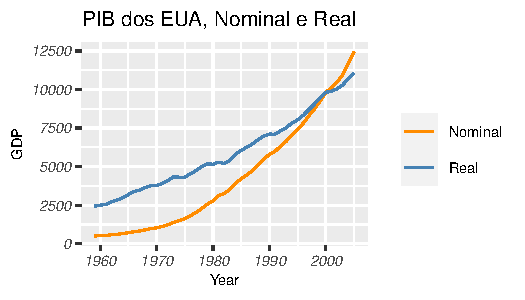
\includegraphics{article_files/figure-latex/unnamed-chunk-28-1} \end{center}

\textbf{b. Denotando o PIB por Y e o tempo por X (medido em uma sequência cronológica em que l represente 1959, 2, 1960 e assim por diante até 47 para 2005), veja se o seguinte modelo ajusta-se aos dados do PIB:}

\[y_t = \beta_1 + \beta_2 x_t + \mu_t\]

Apenas pelo gráfico dá para se notar uma relação entre tempo e variação do PIB. Algo que é bem comum em séries temporais, onde se incluem modelos de regressão para fazer o `forecasting'. Vamos ver se o modelo se adequa bem aos dados.

\begin{itemize}
\tightlist
\item
  PIB Nominal
\end{itemize}

\begin{longtable}[]{@{}ccccc@{}}
\toprule
\begin{minipage}[b]{(\columnwidth - 4\tabcolsep) * \real{0.25}}\centering
~\strut
\end{minipage} & \begin{minipage}[b]{(\columnwidth - 4\tabcolsep) * \real{0.15}}\centering
Estimate\strut
\end{minipage} & \begin{minipage}[b]{(\columnwidth - 4\tabcolsep) * \real{0.18}}\centering
Std. Error\strut
\end{minipage} & \begin{minipage}[b]{(\columnwidth - 4\tabcolsep) * \real{0.14}}\centering
t value\strut
\end{minipage} & \begin{minipage}[b]{(\columnwidth - 4\tabcolsep) * \real{0.17}}\centering
Pr(\textgreater\textbar t\textbar)\strut
\end{minipage}\tabularnewline
\midrule
\endhead
\begin{minipage}[t]{(\columnwidth - 4\tabcolsep) * \real{0.25}}\centering
\textbf{(Intercept)}\strut
\end{minipage} & \begin{minipage}[t]{(\columnwidth - 4\tabcolsep) * \real{0.15}}\centering
-496268\strut
\end{minipage} & \begin{minipage}[t]{(\columnwidth - 4\tabcolsep) * \real{0.18}}\centering
21089\strut
\end{minipage} & \begin{minipage}[t]{(\columnwidth - 4\tabcolsep) * \real{0.14}}\centering
-23.53\strut
\end{minipage} & \begin{minipage}[t]{(\columnwidth - 4\tabcolsep) * \real{0.17}}\centering
6.286e-27\strut
\end{minipage}\tabularnewline
\begin{minipage}[t]{(\columnwidth - 4\tabcolsep) * \real{0.25}}\centering
\textbf{year}\strut
\end{minipage} & \begin{minipage}[t]{(\columnwidth - 4\tabcolsep) * \real{0.15}}\centering
252.6\strut
\end{minipage} & \begin{minipage}[t]{(\columnwidth - 4\tabcolsep) * \real{0.18}}\centering
10.64\strut
\end{minipage} & \begin{minipage}[t]{(\columnwidth - 4\tabcolsep) * \real{0.14}}\centering
23.74\strut
\end{minipage} & \begin{minipage}[t]{(\columnwidth - 4\tabcolsep) * \real{0.17}}\centering
4.367e-27\strut
\end{minipage}\tabularnewline
\bottomrule
\end{longtable}

\begin{longtable}[]{@{}cccc@{}}
\caption{Fitting linear model: ``nominal\_gdp \textasciitilde{} year''}\tabularnewline
\toprule
\begin{minipage}[b]{(\columnwidth - 3\tabcolsep) * \real{0.21}}\centering
Observations\strut
\end{minipage} & \begin{minipage}[b]{(\columnwidth - 3\tabcolsep) * \real{0.31}}\centering
Residual Std. Error\strut
\end{minipage} & \begin{minipage}[b]{(\columnwidth - 3\tabcolsep) * \real{0.11}}\centering
\(R^2\)\strut
\end{minipage} & \begin{minipage}[b]{(\columnwidth - 3\tabcolsep) * \real{0.24}}\centering
Adjusted \(R^2\)\strut
\end{minipage}\tabularnewline
\midrule
\endfirsthead
\toprule
\begin{minipage}[b]{(\columnwidth - 3\tabcolsep) * \real{0.21}}\centering
Observations\strut
\end{minipage} & \begin{minipage}[b]{(\columnwidth - 3\tabcolsep) * \real{0.31}}\centering
Residual Std. Error\strut
\end{minipage} & \begin{minipage}[b]{(\columnwidth - 3\tabcolsep) * \real{0.11}}\centering
\(R^2\)\strut
\end{minipage} & \begin{minipage}[b]{(\columnwidth - 3\tabcolsep) * \real{0.24}}\centering
Adjusted \(R^2\)\strut
\end{minipage}\tabularnewline
\midrule
\endhead
\begin{minipage}[t]{(\columnwidth - 3\tabcolsep) * \real{0.21}}\centering
47\strut
\end{minipage} & \begin{minipage}[t]{(\columnwidth - 3\tabcolsep) * \real{0.31}}\centering
989.5\strut
\end{minipage} & \begin{minipage}[t]{(\columnwidth - 3\tabcolsep) * \real{0.11}}\centering
0.926\strut
\end{minipage} & \begin{minipage}[t]{(\columnwidth - 3\tabcolsep) * \real{0.24}}\centering
0.9244\strut
\end{minipage}\tabularnewline
\bottomrule
\end{longtable}

\begin{itemize}
\tightlist
\item
  PIB Real
\end{itemize}

\begin{longtable}[]{@{}ccccc@{}}
\toprule
\begin{minipage}[b]{(\columnwidth - 4\tabcolsep) * \real{0.25}}\centering
~\strut
\end{minipage} & \begin{minipage}[b]{(\columnwidth - 4\tabcolsep) * \real{0.15}}\centering
Estimate\strut
\end{minipage} & \begin{minipage}[b]{(\columnwidth - 4\tabcolsep) * \real{0.18}}\centering
Std. Error\strut
\end{minipage} & \begin{minipage}[b]{(\columnwidth - 4\tabcolsep) * \real{0.14}}\centering
t value\strut
\end{minipage} & \begin{minipage}[b]{(\columnwidth - 4\tabcolsep) * \real{0.17}}\centering
Pr(\textgreater\textbar t\textbar)\strut
\end{minipage}\tabularnewline
\midrule
\endhead
\begin{minipage}[t]{(\columnwidth - 4\tabcolsep) * \real{0.25}}\centering
\textbf{(Intercept)}\strut
\end{minipage} & \begin{minipage}[t]{(\columnwidth - 4\tabcolsep) * \real{0.15}}\centering
-351335\strut
\end{minipage} & \begin{minipage}[t]{(\columnwidth - 4\tabcolsep) * \real{0.18}}\centering
9070\strut
\end{minipage} & \begin{minipage}[t]{(\columnwidth - 4\tabcolsep) * \real{0.14}}\centering
-38.74\strut
\end{minipage} & \begin{minipage}[t]{(\columnwidth - 4\tabcolsep) * \real{0.17}}\centering
3.332e-36\strut
\end{minipage}\tabularnewline
\begin{minipage}[t]{(\columnwidth - 4\tabcolsep) * \real{0.25}}\centering
\textbf{year}\strut
\end{minipage} & \begin{minipage}[t]{(\columnwidth - 4\tabcolsep) * \real{0.15}}\centering
180.3\strut
\end{minipage} & \begin{minipage}[t]{(\columnwidth - 4\tabcolsep) * \real{0.18}}\centering
4.576\strut
\end{minipage} & \begin{minipage}[t]{(\columnwidth - 4\tabcolsep) * \real{0.14}}\centering
39.39\strut
\end{minipage} & \begin{minipage}[t]{(\columnwidth - 4\tabcolsep) * \real{0.17}}\centering
1.597e-36\strut
\end{minipage}\tabularnewline
\bottomrule
\end{longtable}

\begin{longtable}[]{@{}cccc@{}}
\caption{Fitting linear model: ``real\_gdp \textasciitilde{} year''}\tabularnewline
\toprule
\begin{minipage}[b]{(\columnwidth - 3\tabcolsep) * \real{0.21}}\centering
Observations\strut
\end{minipage} & \begin{minipage}[b]{(\columnwidth - 3\tabcolsep) * \real{0.31}}\centering
Residual Std. Error\strut
\end{minipage} & \begin{minipage}[b]{(\columnwidth - 3\tabcolsep) * \real{0.12}}\centering
\(R^2\)\strut
\end{minipage} & \begin{minipage}[b]{(\columnwidth - 3\tabcolsep) * \real{0.24}}\centering
Adjusted \(R^2\)\strut
\end{minipage}\tabularnewline
\midrule
\endfirsthead
\toprule
\begin{minipage}[b]{(\columnwidth - 3\tabcolsep) * \real{0.21}}\centering
Observations\strut
\end{minipage} & \begin{minipage}[b]{(\columnwidth - 3\tabcolsep) * \real{0.31}}\centering
Residual Std. Error\strut
\end{minipage} & \begin{minipage}[b]{(\columnwidth - 3\tabcolsep) * \real{0.12}}\centering
\(R^2\)\strut
\end{minipage} & \begin{minipage}[b]{(\columnwidth - 3\tabcolsep) * \real{0.24}}\centering
Adjusted \(R^2\)\strut
\end{minipage}\tabularnewline
\midrule
\endhead
\begin{minipage}[t]{(\columnwidth - 3\tabcolsep) * \real{0.21}}\centering
47\strut
\end{minipage} & \begin{minipage}[t]{(\columnwidth - 3\tabcolsep) * \real{0.31}}\centering
425.6\strut
\end{minipage} & \begin{minipage}[t]{(\columnwidth - 3\tabcolsep) * \real{0.12}}\centering
0.9718\strut
\end{minipage} & \begin{minipage}[t]{(\columnwidth - 3\tabcolsep) * \real{0.24}}\centering
0.9712\strut
\end{minipage}\tabularnewline
\bottomrule
\end{longtable}

\textbf{c.~Como você interpretaria }\(\beta_2\)\textbf{?}

Para ambas as variáveis (Nominal e Real), o tempo se mostra estatisticamente significativo (com valor p bastante baixo) e também nos dois modelos a capacidade de explicar variações em Y é alta (demonstrado pelo r²).

\end{document}
